\documentclass[11pt, a4paper]{article}

\renewcommand*\ttdefault{pcr}

\usepackage{float}
\usepackage{scrextend}
\addtokomafont{labelinglabel}{\ttfamily}
\usepackage{color}
\usepackage[top = 3cm, bottom = 3cm, left = 2cm, right = 2cm]{geometry}
\usepackage[francais]{babel}
\usepackage[utf8]{inputenc}
\usepackage{graphicx}
\DeclareGraphicsExtensions{.pdf,.png,.jpg}
\usepackage[colorinlistoftodos]{todonotes}
\usepackage{enumitem}
\usepackage{moreverb}
\usepackage{cancel}
\usepackage{listings}
\lstset{language=C++,
basicstyle=\tt\small,
showstringspaces=false}
\usepackage{titlesec}
\usepackage{color}
\usepackage{fancybox}
\usepackage{svg}
\usepackage[justification=centering]{caption}
\frenchbsetup{StandardLists=true}
%\renewcommand{\familydefault}{\ttdefault}

\title{Compte rendu : TP C++ - Héritage et Polymorphisme}
\author{GUIRAUDOU Bastien et TURPIN Laurent}
\date{\today}

\begin{document}
\maketitle

\section{Introduction}
Dans ce TP, nous devions réaliser un logiciel pour gérer des trajets entre des villes avec
différents moyens de transport. Il devait permettre à l'utilisateur d'ajouter de nouveau trajets,
simples ou composés de plusieurs étapes, à un catalogue, d'afficher ce même catalogue ou encore de
rechercher un trajets parmis ceux existants. Nous avons choisis comme outils de réalisation la
liste chainée, méthode qui nous semblait appropriée car nous l'avions déjà vu et utilisée lors d'un
précédent TP d'algorithmique.

Nous avons essayé, tout au long de notre travail, de faire en sorte que notre programme soit
facilement modulable par la suite, dans le cas ou le cahier des charges viendrait à évoluer.
\section{Descriptions Précises des Classes}
Pour la réalisation de notre TP, nous avons créé cinq classes : Une servant à gérer notre catalogue
de trajet, trois pour la création et la gestion des dit trajets, fonctionnant sous le principe de
l'héritage, et enfin une classe pour définir les éléments de notre liste chainée, puisque nous avons
décidé que notre catalogue fonctionnerait ainsi. Un fichier \texttt{LTIF.cpp} utilise l'ensemble de
ces classes et contient le \texttt{main} du programme, c'est lui qui gère le catalogue.

\subsection{LTIF - Logiciel de Transport IF}
Ce fichier contient le \texttt{main}, ainsi que la gestion de l'interface avec l'utilisateur.
L'interaction entre l'utilisateur et le logiciel se fait directement dans l'invite de commande.

\texttt{MAX\_LENGTH}, un nombre entier constant sert à la création de nos chaines de caractères qui
recevront les entrées de l'utilisateur.

Une fois exécuté, on peut ajouter des trajets au catalogue ou appeler la recherche et l'affichage
de ce catalogue. Un rapide mode d'emploi est affiché au lancement du programme, pour que
l'utilisateur ne soit pas perdu avec l'interface.

\subsection{Catalogue}
Cette classe permet la gestion de notre catalogue de trajet. Elle permet d'ajouter des trajets (à la
fin du catalogue), d'afficher les trajets dans leur ordre d'ajout, ou bien de rechercher un trajet.
Les trajets sont rangés en liste chainée, et la classe contient un pointeur vers le premier élément
et un autre vers le dernier de la liste.\\
\\
\textbf{Attributs :}
\begin{labeling}{first}
\item [first] un pointeur d'élément de liste chainée, pointant vers le premier élément du
catalogue, ou vers \texttt{NULL} si le catalogue est vide.
\item [last] un pointeur d'élément de liste chainée, pointant vers le dernier élément du 
catalogue, ou vers \texttt{NULL} si le catalogue est vide.
\end{labeling}

\subsection{Element}
Cette classe sert a définir les éléments qui composent notre liste chaînée. Un objet de type
\texttt{Element}contient deux pointeurs, un pointant vers un trajet, le deuxième vers
l'élément suivant. Le premier pointe vers un objet de type \texttt{Trajet}, qui peut
être indifféremment un trajet composé ou un trajet simple.\\
\\
\textbf{Attributs :}
\begin{labeling}{next}
\item [next] un pointeur vers un autre objet de type \texttt{Element}, le suivant dans la liste chaînée.
\item [traj] un pointeur vers un objet de type Trajet.
\end{labeling}
Ces éléments servent également à créer des trajets composés, en fonctionnant de la même manière, à
ceci près que lors de la création de trajets composés nous n'utilisons que des trajets simples. En
revanche, en cas de volonté d'évolution, nous pourrons mettre des trajets composés dans d'autres
trajets composés sans que cela pose problème.

\subsection{Trajet}
Cette classe est la classe mère de notre héritage des classes représentant des trajets (cf : Figure
\ref{fig:her}). C'est une classe virtuelle pure, par conséquent il est impossible de créer un objet
de type \texttt{Trajet}, mais cette classe est indispensable à la création d'une chaîne de trajets
polymorphiques.

Cette classe n'a pas d'attributs propres, et aucune de ses méthodes n'est implémentée, elles le sont
dans les classes filles. Nous avons une méthode permettant d'afficher un trajet donné, des getteurs
pour récupérer certain de leurs attributs.
\begin{figure}[H]
    \centering
    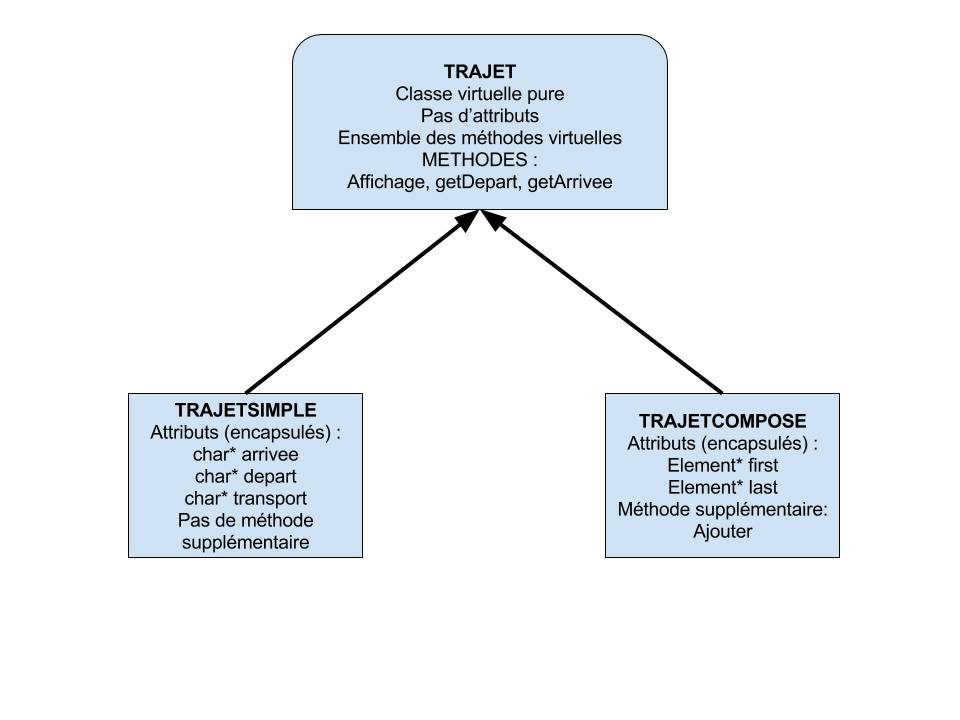
\includegraphics[trim = 30mm 45mm 30mm 0mm, clip, width = 0.7\textwidth]{Heritage}
    \caption{Schéma d'héritage du projet\label{fig:her}}
\end{figure}

\subsection{TrajetSimple}
Cette classe hérite de la classe \texttt{Trajet}. Un objet de type \texttt{TrajetSimple} comporte
une ville de départ, une ville d'arrivée et un moyen de transport. Ce sont des objets de type
\texttt{TrajetSimple} qui sont utilisés pour créer des trajets composés.\\
\\
\textbf{Attributs : }
\begin{labeling}{transport}
\item [arrivee] une chaîne de caractères contenant la ville d'arrivée du trajet.
\item [depart] une chaîne de caractères contenant la ville de départ du trajet.
\item [transport] une chaîne de caractères contenant le moyen de transport.
\end{labeling}
Pour pouvoir récupérer ces attributs, qui sont encapsulés, nous avons créé des getteurs, qui
nous permettent de réutiliser ces attributs en lecture seule sans risques qu'ils soient modifiés
depuis l'extérieur de la classe.

\subsection{TrajetCompose}
Cette classe descend également de la classe \texttt{Trajet}. Un trajet composé fonctionne de la même manière
que notre catalogue, avec une liste chaînée de trajets, qui sont ici tous des trajets simples.
L'ajout se fait en bout de chaine.\\
\\
\textbf{Attributs :}
\begin{labeling}{first}
\item [first] un pointeur d'Element, qui pointe vers le premier trajet simple.
\item [last] un pointeur d'Element, qui pointe vers le dernier trajet simple.
\end{labeling}
Tout comme pour les trajets simples, nous avons des getteurs pour récupérer le départ du premier
trajet simple et l'arrivée du dernier, afin de pouvoir effectuer notre recherche de trajets
correctement.

\section{Structure de données}
Notre structure de données est une liste chaînée. Dans notre objet \texttt{Catalogue}, nous avons deux
pointeurs. Le premier, nommé \texttt{first}, pointe vers le premier élément de notre liste. Le deuxième,
nommé \texttt{last}, pointe vers le dernier élément.
Notre liste est basée sur le principe du First in First out, c'est à dire qu'à l'affichage, le
premier élément inséré est le premier affiché, et que l'insertion se fait en bout de chaine. Nous
n'avons pas de méthode pour supprimer des éléments.

Chaque élément de notre liste chainée est composé de deux pointeurs. Celui nommé \texttt{next} pointe vers
l'élément suivant, et celui nommé \texttt{traj} pointe vers un objet de type trajet. Le pointeur
\texttt{next} du dernier élément pointe vers \texttt{NULL}.

Grâce au système d'héritage, le trajet pointé par un élément peut être indépendamment un trajet
simple ou un trajet composé.

Nos trajets composés sont formés sur le même principe que notre catalogue, et nous avons donc une
nouvelle liste chaînée, avec des pointeurs \texttt{first} et \texttt{last}, et une suite d'éléments. La seule
différence est que dans notre code actuel, l'utilisateur ne peux que former un trajet composé a
partir de trajets simples.

\begin{figure}[H]
    \centering
    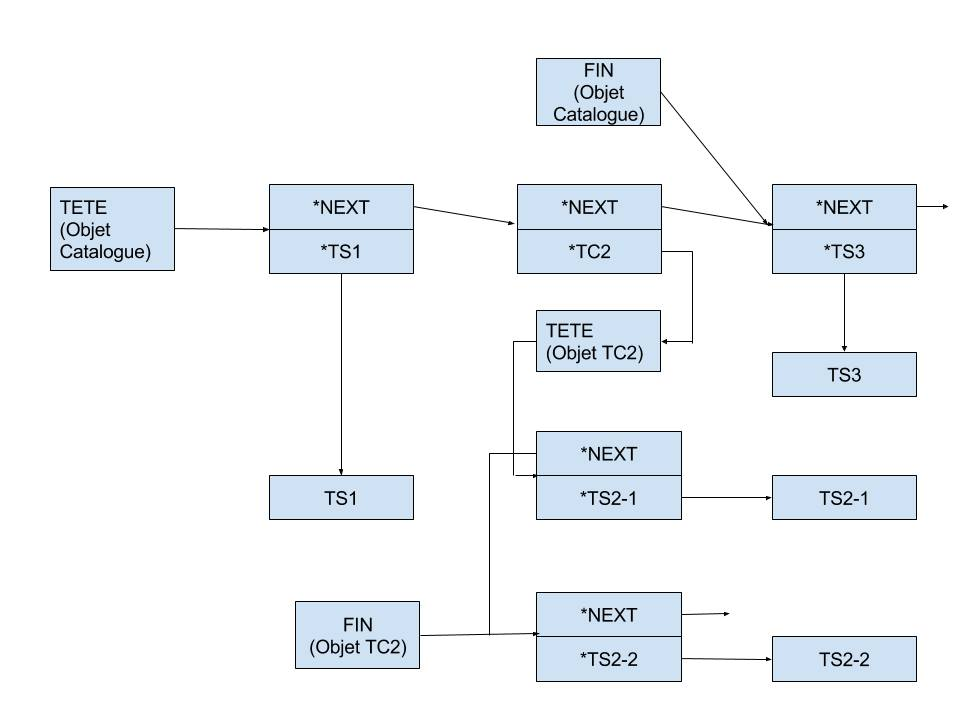
\includegraphics[trim = 0mm 5mm 0mm 5mm, clip, width = 0.8\textwidth]{Struct}
    \caption{Schéma de l'état de la mémoire sur un exemple\label{fig:struct}}
\end{figure}

\section{Liste des classes et méthodes}
\subsection{Trajet}
\begin{lstlisting}
class Trajet;
\end{lstlisting}
La classe \texttt{Trajet} est une classe abstraite décrivant le comportement général d'un trajet.
Chaque méthode de la classe est \texttt{const} car quand un trajet est créé, il ne doit pas être
modifier.

\begin{lstlisting}
virtual void Afficher() const = 0;
\end{lstlisting}
La méthode \texttt{Afficher} permet d'afficher dans la sortie standard la ville de départ du trajet, la
ville d'arrivée et le moyen de transport.

\begin{lstlisting}
virtual const char* getDepart() const = 0;
\end{lstlisting}
La méthode \texttt{getDepart} renvoie la chaine de caractères correspondant à la ville de départ du
trajet

\begin{lstlisting}
virtual const char* getArrivee() const = 0;
\end{lstlisting}
La méthode \texttt{getArrivee} fait la même chose que \texttt{getDepart} mais pour la ville
d'arrivée\\

Les constructeurs et le destructeur de cette classe ne seront pas précisés car c'est une classe
abstraite donc aucun objet de ce type n'est créé.\\

\subsection{TrajetSimple}
\begin{lstlisting}
class TrajetSimple : public Trajet;
\end{lstlisting}
Cette classe hérite de \texttt{Trajet}, elle définit un trajet qui n'a aucune escale, juste un
ville de départ, une ville d'arrivée et un moyen de transport.

\begin{lstlisting}
TrajetSimple (const char* dep, const char* arr, const char* trans);
\end{lstlisting}
Le constructeur prend en paramètre des chaines constantes de caractères pour définir chaque attribut
de la classe.

\begin{lstlisting}
virtual ~TrajetSimple();
\end{lstlisting}
Le destructeur est assez simple, il libère la mémoire pointée par chacun des pointeurs.

\begin{lstlisting}
void Afficher() const;
\end{lstlisting}
Affiche sur la sortie standard toutes les caractéristiques de la classe de la manière suivante :\\
"De \texttt{[Ville de départ]} à \texttt{[Ville d'arrivée]} en \texttt{[Moyen de Transport]}\\
Il n'y a pas de retour à la ligne à la fin, le formatage de l'affichage sera mieux géré par le
catalogue.

\begin{lstlisting}
const char* getDepart() const;
\end{lstlisting}
Cette méthode renvoie la chaine de caractères \texttt{depart} correspondant à la ville de départ du
trajet simple.

\begin{lstlisting}
const char* getArrivee() const;
\end{lstlisting}
Cette méthode renvoie la chaine de caractères \texttt{arrivee} correspondant à la ville d'arrivée du
trajet simple.\\

\subsection{Element}
\begin{lstlisting}
classe Element;
\end{lstlisting}
Cette classe défini les objets représentant les maillons d'une liste chaînée composée d'objets de
type \texttt{Trajet}.

\begin{lstlisting}
Element (const Trajet* tr);
\end{lstlisting}
Le constructeur de la classe prend en paramètre un pointeur vers un \texttt{Trajet} et l'assigne au pointeur
\texttt{traj}. Comme le type de ce pointeur est constant, il suffit de faire une affectation
classique. Cependant, il faut faire attention à ne pas modifier le pointeur utilisé pour la
construction après coup. Le pointeur vers le maillon suivant et initialisé à \texttt{NULL} ce qui
nous permet de connaître la fin de la liste.

\begin{lstlisting}
virtual ~Element();
\end{lstlisting}
Le Destructeur ne "détruit" que son trajet associé, c'est la classe qui gérera la liste qui fera le
reste.

\begin{lstlisting}
const Trajet* getTraj() const;
\end{lstlisting}
Cette méthode renvoie le pointeur \texttt{traj} du maillon. Pour ne pas compromettre l'intégrité du
maillon et ne pas modifier son information utile, la méthode est \texttt{const} et surtout il faut
directement utiliser une méthode associée au trajet.

\begin{lstlisting}
void setNext(Element* n);
\end{lstlisting}
Cette méthode permet de modifier le pointeur \texttt{next} de la classe pour notamment ajouter
\texttt{n} comme prochain maillon de la chaine.

\begin{lstlisting}
Element* getNext() const;
\end{lstlisting}
Cette méthode renvoie le pointeur \texttt{next} servant à parcourir la liste chaînée.\\

\subsection{Trajet Compose}
\begin{lstlisting}
class TrajetCompose : public Trajet;
\end{lstlisting}
Cette classe hérite également de \texttt{Trajet}, elle définit un trajet pouvant avoir de multiples
escales. Elle est implémentée comme une liste chainée utilisant les objets de type \texttt{Element}
comme maillons de la liste. Elle contient deux pointeurs, un sur le début de la liste et un sur la
fin . Pour ce TP, ce sera une liste chaînées avec exclusivement des objets de type
\texttt{TrajetSimple}.

\begin{lstlisting}
TrajetCompse();
\end{lstlisting}
Le constructeur initialise les deux pointeurs à \texttt{NULL}, c'est donc l'état d'une liste vide.

\begin{lstlisting}
virtual ~TrajetCompose();
\end{lstlisting}
Le destructeur doit donc se charger de libérer la mémoire pour chaque maillon grâce à une simple
boucle.

\begin{lstlisting}
void Afficher() const;
\end{lstlisting}
Cette méthode utilise la méthode \texttt{Afficher} de chaque maillon de la liste séparé par un
tiret "-".

\begin{lstlisting}
const char* getDepat() const;
\end{lstlisting}
Cette méthode utilise la méthode \texttt{getDepart} du premier maillon de la liste.

\begin{lstlisting}
const char* getArriverr() const;
\end{lstlisting}
Cette méthode utilise la méthode \texttt{getArrivee} du dernier maillon de la liste.

\begin{lstlisting}
void Ajouter(Trajet* tr);
\end{lstlisting}
Cette méthode crée un nouveau maillon avec \texttt{tr} et le place en fin de la liste. Il faut
absolument que la ville de départ d'un maillon corresponde à la ville d'arrivée du maillon précédent
pour que le trajet soit licite.\\

\subsection{Catalogue}
\begin{lstlisting}
classe Catalogue;
\end{lstlisting}
Cette classe représente le catalogue complet des trajets. Elle est implémentée comme une liste chaînée dont les
maillons sont des objets de type \texttt{Trajet}. Elle contient donc deux pointeurs, une pour le
début et un pour la fin de la liste.

\begin{lstlisting}
Catalogue();
\end{lstlisting}
Le constructeur initialise les deux pointeurs à \texttt{NULL}, c'est donc l'état d'un catalogue
vide.

\begin{lstlisting}
virtual ~Catalogue();
\end{lstlisting}
Le destructeur doit se charger de libérer la mémoire de chaque maillons.

\begin{lstlisting}
void Afficher() const;
\end{lstlisting}
Cette méthode affiche à la sortie standard les trajets du catalogue ligne par ligne en utilisant la
méthodes \texttt{Afficher} de chaque maillon.

\begin{lstlisting}
void Ajouter(const Trajet* tr);
\end{lstlisting}
Cette méthode crée un nouveau maillon avec le paramètre \texttt{tt} et le place à la fin de la liste.

\begin{lstlisting}
void Rechercher(const char* dep, const char* arr) const;
\end{lstlisting}
Cette méthode affiche ligne par ligne tous les trajets qui ont comme ville de départ le paramètre
\texttt{dep} et comme ville d'arrivée le paramètre \texttt{arr}.
Sachant qu'un trajet doit toujours être pris au complet, on ne peut pas interrompre un trajet
composé.

\section{Problèmes rencontrés et axes d'amélioration}
\subsection{Problèmes}
Durant ce TP, nous avons eu des problèmes sur la façon de définir \texttt{const} certains attributs.
En effet le fait de l'avoir fait un peu tard dans la réalisation a provoqué une réaction en chaîne
où nous devions revoir les méthodes impactées par le changement. Cependant la définition en
\texttt{const} de certains attributs (ceux des trajets simples) leur donnait un comportement peu
désirable : on ne pouvait les définir qu'avec une affectation classique avec un autre pointeur. Donc
si on changeait ce dernier pointeur, l'attribut changeait également.

De plus, réaliser la recherche avancée a été bien plus dur que prévu. L'algorithme fonctionne bel
et bien grâce à une récursivité mais génère des fuites de mémoire venant de la créations de
pointeurs qui pointent sur des objets déjà présents et qui ne doivent surtout pas être détruits. On
de peut donc pas appliquer de \texttt{delete} sur ces nouveaux pointeurs au risque de corrompre les
données du catalogue.

\subsection{Améliorations}
Pour améliorer ce programme, on peut déjà étendre le type des éléments contenus dans un trajet
composé à des trajets de tout types (simple et composé). En réalité, l'opération est déjà faisable
avec le code actuel.

Ensuite, on pourrait très bien n'avoir que des objets de types
\texttt{TrajetCompose} dans le catalogue, avec des trajets composés ne comprenant qu'un seul trajet
simple par exemple. Cela réduirait certaines redondances dans le code du fichier \texttt{LTIF.cpp}

On pourrait ajouter des méthodes pour retirer des trajet dans le catalogue ou filtrer les recherches
suivant les moyens de transport, ou bien en trajet direct, ou bien en imposant des escale.
On pourrait aussi assurer l'unicité des trajets dans le catalogue, le fait de ne pas faire de boucle
avec les trajets composés.

Enfin une interface graphique sera toujours bien appréciée.
\newpage
\section{Annexes : code source}
\subsection{Trajet}
\lstinputlisting[frame=single, numbers=left, numbersep=5pt, stepnumber=1, title=\lstname]{Trajet.h}
\subsection{TrajetSimple}
\lstinputlisting[frame=single, numbers=left, numbersep=5pt, stepnumber=1, title=\lstname]{TrajetSimple.h}
\lstinputlisting[frame=single, numbers=left, numbersep=5pt, stepnumber=1, title=\lstname]{TrajetSimple.cpp}
\newpage
\subsection{TrajetCompose}
\lstinputlisting[frame=single, numbers=left, numbersep=5pt, stepnumber=1, title=\lstname]{TrajetCompose.h}
\lstinputlisting[frame=single, numbers=left, numbersep=5pt, stepnumber=1, title=\lstname]{TrajetCompose.cpp}
\subsection{Element}
\lstinputlisting[frame=single, numbers=left, numbersep=5pt, stepnumber=1, title=\lstname]{Element.h}
\lstinputlisting[frame=single, numbers=left, numbersep=5pt, stepnumber=1, title=\lstname]{Element.cpp}
\newpage
\subsection{Catalogue}
\lstinputlisting[frame=single, numbers=left, numbersep=5pt, stepnumber=1, title=\lstname]{Catalogue.h}
\lstinputlisting[frame=single, numbers=left, numbersep=5pt, stepnumber=1, title=\lstname]{Catalogue.cpp}
\newpage
\subsection{Tests unitaires}
\lstinputlisting[frame=single, numbers=left, numbersep=5pt, stepnumber=1, title=\lstname]{Test.cpp}
\subsection{LTIF}
\lstinputlisting[frame=single, numbers=left, numbersep=5pt, stepnumber=1, title=\lstname]{LTIF.cpp}
\end{document}
